\documentclass{standalone}
\usepackage{tikz}
\usetikzlibrary{calc, shapes.geometric, arrows.meta, positioning, fit, decorations.pathreplacing}

\begin{document}
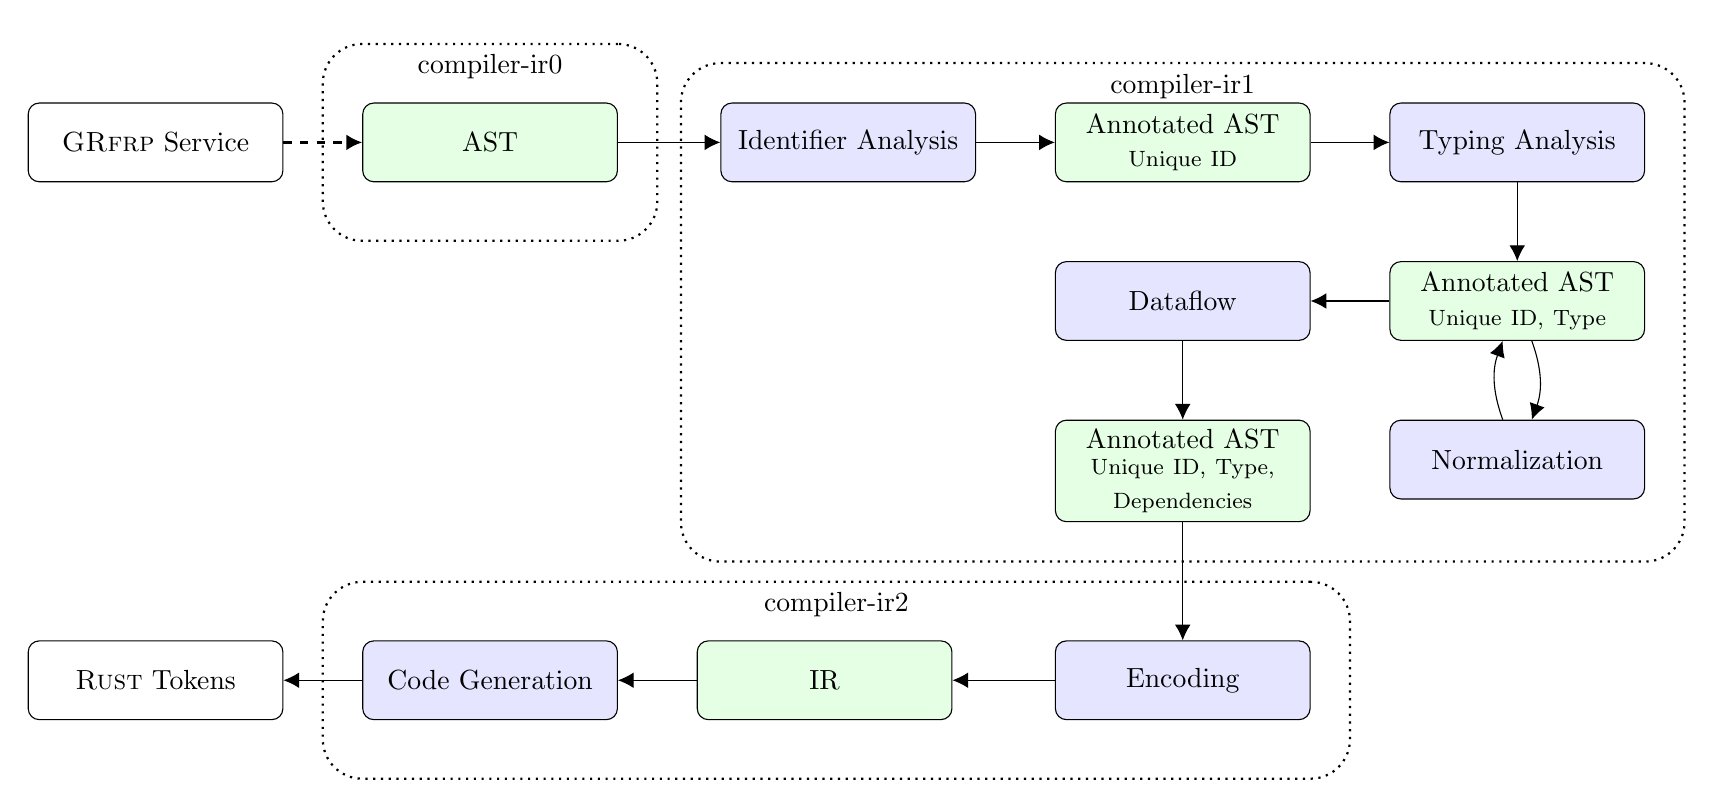
\begin{tikzpicture}[
    node distance=1cm,
    every node/.style={
            rectangle,
            rounded corners,
            draw,
            text width=3cm,
            text centered,
            minimum height=1cm
        },
    arrow/.style={-{Latex[length=2mm, width=2mm]}},
    crate_border/.style={
            dotted,
            thick,
            rounded corners=5mm,
            inner sep=5mm,
            minimum height=2.5cm,
            minimum width=3.5cm
        },
    process_block/.style={fill=blue!10},
    data_block/.style={fill=green!10},
    ]

    % --- Input ---
    \node (grust_code) {\textsc{GRfrp} Service};

    % --- Frontend ---
    \node (ast) [data_block, right=of grust_code] {AST};
    \node (id_analysis) [process_block, right=1.3cm of ast] {Identifier Analysis};
    \node (id_ast) [data_block, right=of id_analysis] {Annotated AST\\ {\footnotesize Unique ID}};
    \node (type_analysis) [process_block, right= of id_ast] {Typing Analysis};
    \node (type_ast) [data_block, below=of type_analysis] {Annotated AST\\ {\footnotesize Unique ID, Type}};
    \node (normalization) [process_block, below= of type_ast] {Normalization};
    \node (dataflow) [process_block, left=of type_ast] {Dataflow};
    \node (deps_ast) [data_block, below=of dataflow] {Annotated AST\\ {\footnotesize Unique ID, Type,\\ Dependencies}};

    % --- Backend ---
    \node (encoding) [process_block, below=1.5cm of deps_ast] {Encoding};
    \node (target_ir) [data_block, left=1.3cm of encoding] {IR};
    \node (codegen) [process_block, left=of target_ir] {Code Generation};
    \node (rust_tokens) [left=of codegen] {\textsc{Rust} Tokens};

    % --- Arrows ---
    \draw[arrow, dashed, thick] (grust_code) -- (ast);
    \draw[arrow] (ast) -- (id_analysis);
    \draw[arrow] (id_analysis) -- (id_ast);
    \draw[arrow] (id_ast) -- (type_analysis);
    \draw[arrow] (type_analysis) -- (type_ast);
    \draw[arrow] (type_ast) to [bend left=20] (normalization);
    \draw[arrow] (normalization) to [bend left=20] (type_ast);
    \draw[arrow] (type_ast) -- (dataflow);
    \draw[arrow] (dataflow) -- (deps_ast);
    \draw[arrow] (deps_ast) -- (encoding);
    \draw[arrow] (encoding) -- (target_ir);
    \draw[arrow] (target_ir) -- (codegen);
    \draw[arrow] (codegen) -- (rust_tokens);

    % --- GRust Compiler Crates (Overlapping with Frontend/Backend) ---
    \node[crate_border,
        fit=(ast),
        label={[anchor=north, yshift=0.2cm]north:compiler-ir0}] (ir0_border) {};

    \node[crate_border,
        fit=(id_analysis) (id_ast) (type_analysis) (type_ast) (normalization) (dataflow) (deps_ast),
        label={[anchor=north, yshift=0.2cm]north:compiler-ir1}] (ir1_border) {};

    \node[crate_border,
        fit=(encoding) (target_ir) (codegen),
        label={[anchor=north, yshift=0.2cm]north:compiler-ir2}] (ir2_border) {};

    % % --- Frontend/Backend Labels ---
    % \node [label_block, above=1cm of codegen, font=\large] (backend) {Backend};
    % \node [label_block, above=0.5cm of backend, font=\large] (frontend) {Frontend};

    % % --- Dashed Line ---
    % \coordinate (P) at ($(backend)!0.5!(frontend)$);
    % \draw[dashed, thick]
    % let \p1 = (P) in
    % let \p2 = (normalization) in
    % let \p3 = (rust_tokens) in
    % ($(0,\y1)+(\x2+1.5cm,0)$) -- ($(0,\y1)+(\x3-1cm,0)$);

\end{tikzpicture}
\end{document}
